\documentclass{standalone}
\usepackage{tikz}
\usetikzlibrary{patterns, positioning}


\begin{document}
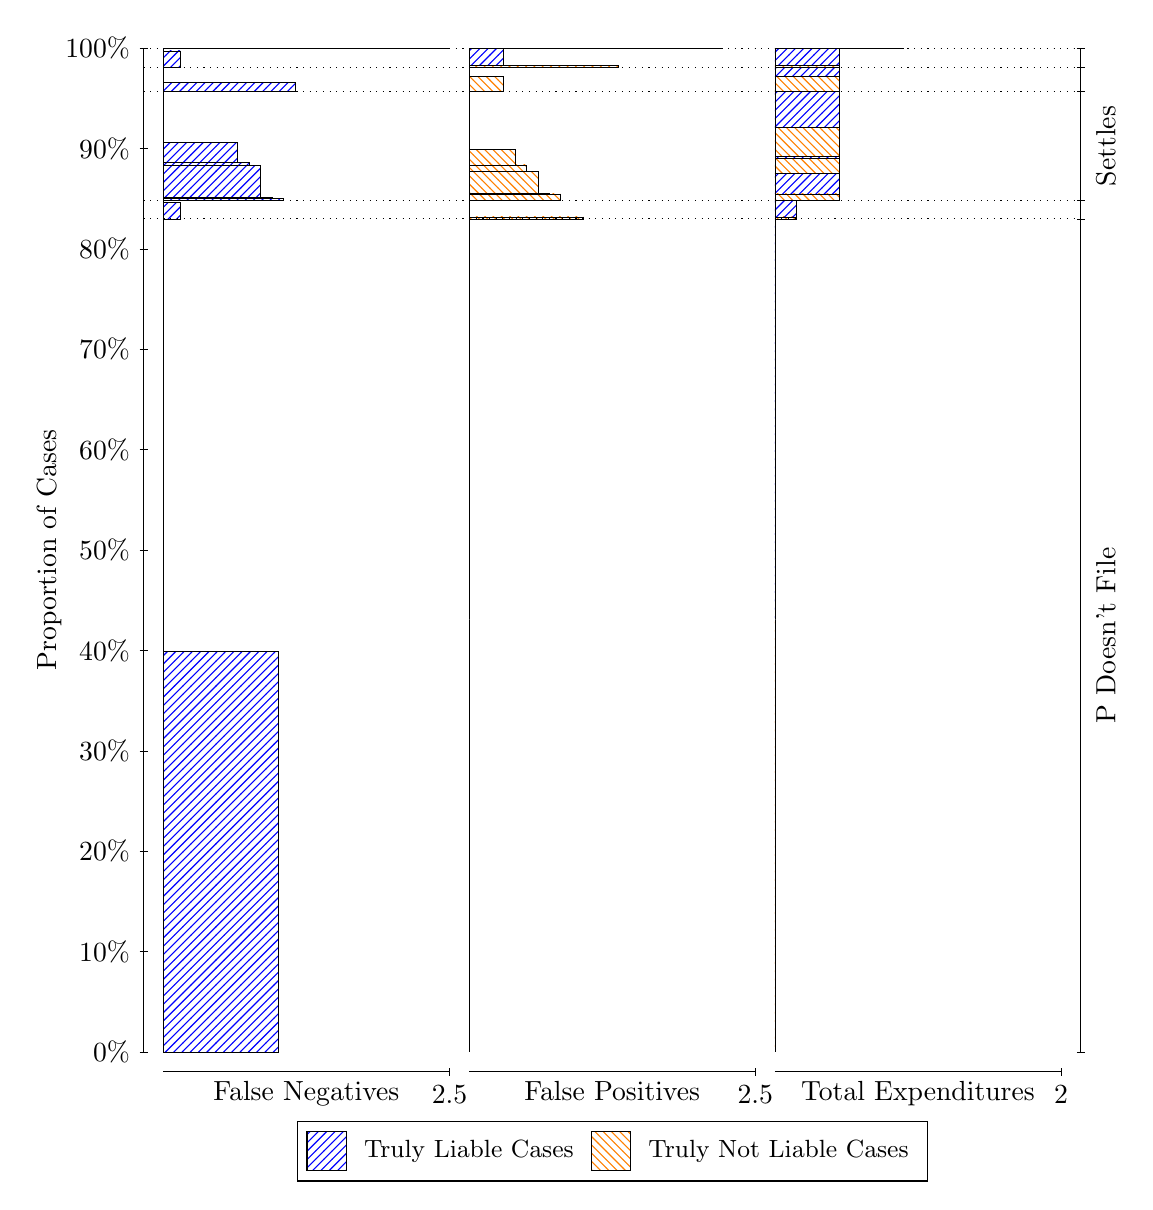
\begin{tikzpicture}
\draw[black, very thin] (1.5,1.75) -- (1.5,14.5);
\node[rotate=90, text=black, anchor=center] at (0.3, 8.125) {Proportion of Cases};
\draw[black, very thin] (1.45,1.75) -- (1.55,1.75);
\node[text=black, anchor=east] at (1.45, 1.75) {0\%};
\draw[black, very thin] (1.45,3.025) -- (1.55,3.025);
\node[text=black, anchor=east] at (1.45, 3.025) {10\%};
\draw[black, very thin] (1.45,4.3) -- (1.55,4.3);
\node[text=black, anchor=east] at (1.45, 4.3) {20\%};
\draw[black, very thin] (1.45,5.575) -- (1.55,5.575);
\node[text=black, anchor=east] at (1.45, 5.575) {30\%};
\draw[black, very thin] (1.45,6.85) -- (1.55,6.85);
\node[text=black, anchor=east] at (1.45, 6.85) {40\%};
\draw[black, very thin] (1.45,8.125) -- (1.55,8.125);
\node[text=black, anchor=east] at (1.45, 8.125) {50\%};
\draw[black, very thin] (1.45,9.4) -- (1.55,9.4);
\node[text=black, anchor=east] at (1.45, 9.4) {60\%};
\draw[black, very thin] (1.45,10.675) -- (1.55,10.675);
\node[text=black, anchor=east] at (1.45, 10.675) {70\%};
\draw[black, very thin] (1.45,11.95) -- (1.55,11.95);
\node[text=black, anchor=east] at (1.45, 11.95) {80\%};
\draw[black, very thin] (1.45,13.225) -- (1.55,13.225);
\node[text=black, anchor=east] at (1.45, 13.225) {90\%};
\draw[black, very thin] (1.45,14.5) -- (1.55,14.5);
\node[text=black, anchor=east] at (1.45, 14.5) {100\%};

\draw[black, very thin] (13.4,1.75) -- (13.4,14.5);
\draw[black, very thin] (13.35,1.75) -- (13.45,1.75);
\node[anchor=west] at (13.35, 1.75) {};
\draw[black, very thin] (13.35,12.33) -- (13.45,12.33);
\node[anchor=west] at (13.35, 12.33) {};
\draw[black, very thin] (13.35,12.566) -- (13.45,12.566);
\node[anchor=west] at (13.35, 12.566) {};
\draw[black, very thin] (13.35,13.946) -- (13.45,13.946);
\node[anchor=west] at (13.35, 13.946) {};
\draw[black, very thin] (13.35,14.253) -- (13.45,14.253);
\node[anchor=west] at (13.35, 14.253) {};
\draw[black, very thin] (13.35,14.491) -- (13.45,14.491);
\node[anchor=west] at (13.35, 14.491) {};
\draw[black, very thin] (13.35,14.494) -- (13.45,14.494);
\node[anchor=west] at (13.35, 14.494) {};
\draw[black, very thin] (13.35,14.5) -- (13.45,14.5);
\node[anchor=west] at (13.35, 14.5) {};

\draw[black, very thin, pattern color=blue, pattern=north east lines] (1.75,1.75) rectangle (3.2033,6.8398);
\draw[black, very thin, pattern color=orange, pattern=north west lines] (1.75,6.8398) rectangle (1.75,12.33);
\draw[black, very thin, pattern color=blue, pattern=north east lines] (1.75,12.33) rectangle (1.968,12.542);
\draw[black, very thin, pattern color=orange, pattern=north west lines] (1.75,12.542) rectangle (1.75,12.566);
\draw[black, very thin, pattern color=blue, pattern=north east lines] (1.75,12.566) rectangle (3.276,12.59);
\draw[black, very thin, pattern color=blue, pattern=north east lines] (1.75,12.59) rectangle (3.1307,12.603);
\draw[black, very thin, pattern color=blue, pattern=north east lines] (1.75,12.603) rectangle (2.9853,13.008);
\draw[black, very thin, pattern color=blue, pattern=north east lines] (1.75,13.008) rectangle (2.84,13.044);
\draw[black, very thin, pattern color=blue, pattern=north east lines] (1.75,13.044) rectangle (2.6947,13.305);
\draw[black, very thin, pattern color=orange, pattern=north west lines] (1.75,13.305) rectangle (1.75,13.946);
\draw[black, very thin, pattern color=blue, pattern=north east lines] (1.75,13.946) rectangle (3.4213,14.064);
\draw[black, very thin, pattern color=orange, pattern=north west lines] (1.75,14.064) rectangle (1.75,14.253);
\draw[black, very thin, pattern color=blue, pattern=north east lines] (1.75,14.253) rectangle (1.968,14.464);
\draw[black, very thin, pattern color=orange, pattern=north west lines] (1.75,14.464) rectangle (1.75,14.491);
\draw[black, very thin, pattern color=blue, pattern=north east lines] (1.75,14.491) rectangle (5.3833,14.492);
\draw[black, very thin, pattern color=orange, pattern=north west lines] (1.75,14.492) rectangle (1.75,14.494);
\draw[black, very thin, pattern color=orange, pattern=north west lines] (1.75,14.494) rectangle (1.75,14.495);
\draw[black, very thin, pattern color=blue, pattern=north east lines] (1.75,14.495) rectangle (1.75,14.5);
\draw[black, very thin, pattern color=orange, pattern=north west lines] (5.6333,1.75) rectangle (5.6333,7.2403);
\draw[black, very thin, pattern color=blue, pattern=north east lines] (5.6333,7.2403) rectangle (5.6333,12.33);
\draw[black, very thin, pattern color=orange, pattern=north west lines] (5.6333,12.33) rectangle (7.0867,12.355);
\draw[black, very thin, pattern color=blue, pattern=north east lines] (5.6333,12.355) rectangle (5.6333,12.566);
\draw[black, very thin, pattern color=orange, pattern=north west lines] (5.6333,12.566) rectangle (6.796,12.647);
\draw[black, very thin, pattern color=orange, pattern=north west lines] (5.6333,12.647) rectangle (6.6507,12.65);
\draw[black, very thin, pattern color=orange, pattern=north west lines] (5.6333,12.65) rectangle (6.5053,12.929);
\draw[black, very thin, pattern color=orange, pattern=north west lines] (5.6333,12.929) rectangle (6.36,13.016);
\draw[black, very thin, pattern color=orange, pattern=north west lines] (5.6333,13.016) rectangle (6.2147,13.208);
\draw[black, very thin, pattern color=blue, pattern=north east lines] (5.6333,13.208) rectangle (5.6333,13.946);
\draw[black, very thin, pattern color=orange, pattern=north west lines] (5.6333,13.946) rectangle (6.0693,14.135);
\draw[black, very thin, pattern color=blue, pattern=north east lines] (5.6333,14.135) rectangle (5.6333,14.253);
\draw[black, very thin, pattern color=orange, pattern=north west lines] (5.6333,14.253) rectangle (7.5227,14.28);
\draw[black, very thin, pattern color=blue, pattern=north east lines] (5.6333,14.28) rectangle (6.0693,14.491);
\draw[black, very thin, pattern color=orange, pattern=north west lines] (5.6333,14.491) rectangle (5.6333,14.492);
\draw[black, very thin, pattern color=blue, pattern=north east lines] (5.6333,14.492) rectangle (5.6333,14.494);
\draw[black, very thin, pattern color=orange, pattern=north west lines] (5.6333,14.494) rectangle (8.8307,14.495);
\draw[black, very thin, pattern color=blue, pattern=north east lines] (5.6333,14.495) rectangle (7.3773,14.5);
\draw[black, very thin, pattern color=orange, pattern=north west lines] (9.5167,1.75) rectangle (9.5167,7.2403);
\draw[black, very thin, pattern color=blue, pattern=north east lines] (9.5167,7.2403) rectangle (9.5167,12.33);
\draw[black, very thin, pattern color=orange, pattern=north west lines] (9.5167,12.33) rectangle (9.7892,12.355);
\draw[black, very thin, pattern color=blue, pattern=north east lines] (9.5167,12.355) rectangle (9.7892,12.566);
\draw[black, very thin, pattern color=orange, pattern=north west lines] (9.5167,12.566) rectangle (10.334,12.647);
\draw[black, very thin, pattern color=blue, pattern=north east lines] (9.5167,12.647) rectangle (10.334,12.907);
\draw[black, very thin, pattern color=orange, pattern=north west lines] (9.5167,12.907) rectangle (10.334,13.1);
\draw[black, very thin, pattern color=blue, pattern=north east lines] (9.5167,13.1) rectangle (10.334,13.123);
\draw[black, very thin, pattern color=orange, pattern=north west lines] (9.5167,13.123) rectangle (10.334,13.492);
\draw[black, very thin, pattern color=blue, pattern=north east lines] (9.5167,13.492) rectangle (10.334,13.946);
\draw[black, very thin, pattern color=orange, pattern=north west lines] (9.5167,13.946) rectangle (10.334,14.135);
\draw[black, very thin, pattern color=blue, pattern=north east lines] (9.5167,14.135) rectangle (10.334,14.253);
\draw[black, very thin, pattern color=orange, pattern=north west lines] (9.5167,14.253) rectangle (10.334,14.28);
\draw[black, very thin, pattern color=blue, pattern=north east lines] (9.5167,14.28) rectangle (10.334,14.491);
\draw[black, very thin, pattern color=orange, pattern=north west lines] (9.5167,14.491) rectangle (11.152,14.492);
\draw[black, very thin, pattern color=blue, pattern=north east lines] (9.5167,14.492) rectangle (11.152,14.494);
\draw[black, very thin, pattern color=orange, pattern=north west lines] (9.5167,14.494) rectangle (11.152,14.495);
\draw[black, very thin, pattern color=blue, pattern=north east lines] (9.5167,14.495) rectangle (11.152,14.5);
\draw[black, dotted] (1.5,12.33) -- (13.4,12.33);
\draw[black, dotted] (1.5,12.566) -- (13.4,12.566);
\draw[black, dotted] (1.5,13.946) -- (13.4,13.946);
\draw[black, dotted] (1.5,14.253) -- (13.4,14.253);
\draw[black, dotted] (1.5,14.491) -- (13.4,14.491);
\draw[black, dotted] (1.5,14.494) -- (13.4,14.494);
\draw[black, very thin] (1.75,1.5) -- (5.3833,1.5);
\node[text=black, anchor=north] at (3.5667, 1.5) {False Negatives};
\draw[black, very thin] (5.3833,1.45) -- (5.3833,1.55);
\node[text=black, anchor=north] at (5.3833, 1.45) {2.5};

\draw[black, very thin] (5.6333,1.5) -- (9.2667,1.5);
\node[text=black, anchor=north] at (7.45, 1.5) {False Positives};
\draw[black, very thin] (9.2667,1.45) -- (9.2667,1.55);
\node[text=black, anchor=north] at (9.2667, 1.45) {2.5};

\draw[black, very thin] (9.5167,1.5) -- (13.15,1.5);
\node[text=black, anchor=north] at (11.333, 1.5) {Total Expenditures};
\draw[black, very thin] (13.15,1.45) -- (13.15,1.55);
\node[text=black, anchor=north] at (13.15, 1.45) {2};

\node[text=black, centered, rotate=90] at (13.72, 7.0401) {P Doesn't File};

\node[text=black, centered, rotate=90] at (13.72, 13.256) {Settles};





\draw (7.449999999999999,1.5) node[draw=none] (baseCoordinate) {};
\begin{scope}[align=center]
        \matrix[scale=0.5, draw=black, below=0.5cm of baseCoordinate, nodes={draw}, column sep=0.1cm]{
            \node[rectangle, draw, minimum width=0.5cm, minimum height=0.5cm, pattern color=blue, pattern=north east lines] {}; &
            \node[draw=none, font=\small, text=black] (B) {Truly Liable Cases}; &
            \node[rectangle, draw, minimum width=0.5cm, minimum height=0.5cm, pattern color=orange, pattern=north west lines] {}; &
            \node[draw=none, font=\small, text=black] (B) {Truly Not Liable Cases}; \\
            };
\end{scope}

\end{tikzpicture}
\end{document}